\begin{center}
    

{
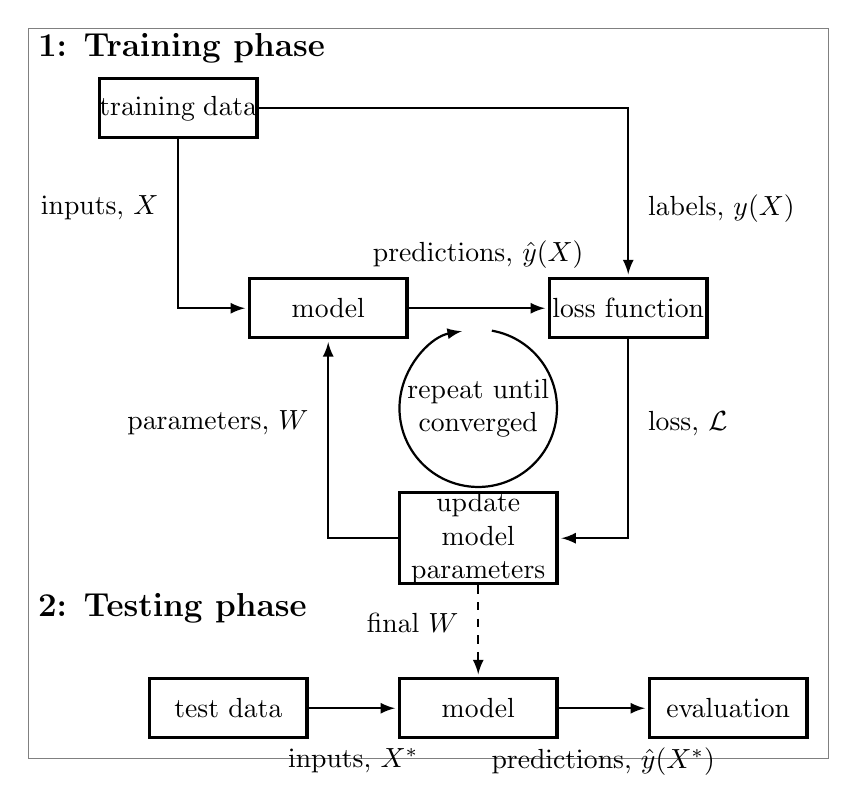
\begin{tikzpicture}[shorten >=1pt,draw=black!50, x = 1 in, y = 1 in,  node distance=20pt,>=latex]
\tikzset{tbox/.style={draw, text badly centered, very thick, black, rectangle, inner sep=0, minimum width = 2.0 cm, minimum height = 0.75 cm}}
\def\circledarrow#1#2#3{ % #1 Style, #2 Center, #3 Radius
\draw[#1,->] (#2) +(80:#3) arc(80:-260:#3);}
\draw[draw=gray, use as bounding box](-2.5,-2.25) rectangle (1.5,1.40);
%% define coordinate grid 
\def \xfarleft {-1.750}
\def \xleft {-1.0}
\def \xmid {-0.25}
\def \xright {0.5}
\def \ytop {1.0}
\def \ymid {0}
\def \ybot {-1.15}
\def \yphasetwo {-2.0}
\def \xlabeloffset {0.05}
\def \ylabeloffset {0.15}

%% training phase 
\node[anchor=west] (part1) at (-2.5,1.30) {\large \textbf{1: Training phase}};
\node [tbox,minimum width=2.0 cm, text width = 2.0 cm] (traindata) at (\xfarleft,\ytop) {training data};
\node [] (traindatay) at (\xright,\ytop) {};
\node [tbox,minimum width=2.0 cm, text width = 2.0 cm] (modelparams) at (\xmid,\ybot) {update model parameters};
\node [tbox,minimum width=2.0 cm, text width = 2.0 cm] (model) at (\xleft,\ymid) {model};
\node [tbox,minimum width=2.0 cm, text width = 2.0 cm] (lossf) at (\xright,\ymid) {loss function};
% paths
\draw [thick, black,->] (traindata.south) |-  (model.west);
\draw [thick, black,->] (model.east) to node [midway,above,label={[label distance=0.15cm]90:}] {} (lossf.west);
\draw [thick, black,->] (traindata.east) -- (traindatay.center) -- (lossf.north);
\draw [thick, black,->] (lossf.south) |- (modelparams.east);
\draw [thick, black,->] (modelparams.west) -| (model.south);

% node labels
\node[anchor=east] (inputslab) at (\xfarleft - \xlabeloffset,0.5*\ymid + 0.5*\ytop)  {inputs, $X$};
\node[anchor=west] (labslab) at (\xright + \xlabeloffset,0.5*\ymid + 0.5*\ytop)  {labels, $y(X)$};
\node[anchor=east] (paramslab) at (\xleft - \xlabeloffset,0.5*\ymid + 0.5*\ybot)  {parameters, $W$};
\node[anchor=west] (errorslab) at (\xright + \xlabeloffset,0.5*\ymid + 0.5*\ybot)  {loss, $\mathcal{L}$};
\node[anchor=south] (predslab) at (\xmid,\ymid + \ylabeloffset)  {predictions, $\hat{y}(X)$};

% loop
\node[text width = 2.0cm,text badly centered] (text) at (\xmid,-0.5) {repeat until converged};
\circledarrow{thick, black}{text}{1cm};
%% testing phase %%
\node[anchor=west] (part2) at (-2.5,-1.5) {\large \textbf{2: Testing phase}};
\node [tbox,minimum width=2.0 cm, text width = 2.0 cm] (testdata) at (\xmid-1.25,\yphasetwo) {test data};
\node [tbox,minimum width=2.0 cm, text width = 2.0 cm] (model2) at (\xmid,\yphasetwo) {model};
\node [tbox,minimum width=2.0 cm, text width = 2.0 cm] (evalf) at (\xmid +1.25,\yphasetwo) {evaluation};
% paths
\draw [thick, black,->] (testdata.east) --  (model2.west);
\draw [thick, black,->] (model2.east) --  (evalf.west);
\draw [thick, black,->,dashed] (modelparams.south) --  (model2.north);
% node lables
\node[anchor=east] (transferlab) at (\xmid - \xlabeloffset,0.5*\ybot + 0.5*\yphasetwo)  {final $W$};
\node[anchor=north] (testxlab) at (\xmid-0.625,\yphasetwo - \ylabeloffset)  {inputs, $X^*$};
\node[anchor=north] (testpredslab) at (\xmid + 0.625,\yphasetwo - \ylabeloffset)  {predictions, $\hat{y}(X^*)$};
\end{tikzpicture}
}
\end{center}
